\chapter{The \chips R\&D Project} %%%%%%%%%%%%%%%%%%%%%%%%%%%%%%%%%%%%%%%%%%%%%%%%%%%%%%%%%%%%%%%%
\label{chap:chips}

\begin{comment} % PLAN %%%%%%%%%%%%%%%%%%%%%%%%%%%%%%%%%%%%%%%%%%%%%%%%%%%%%%%%%%%%%%%%%%%%%%%%%%%
THE CHIPS CONCEPT
- We need cheap large detectors
- We need to use commercially availiable hardware
- We need to be able to fit detector size/scalability to availiable funds
- The CHIPS-M detector

THE CHIPS-5 DETECTOR
- Detector structure
- Detector instrumentation
- Detector deployment
- Current status

MONTE CARLO EVENT GENERATION AND SIMULATION
- Beam event generation
- Cosmic event generation
- Detector simulation
\end{comment}

\section{The \chips concept} %%%%%%%%%%%%%%%%%%%%%%%%%%%%%%%%%%%%%%%%%%%%%%%%%%%%%%%%%%%%%%%%%%%%%
\label{sec:chips_concept} %%%%%%%%%%%%%%%%%%%%%%%%%%%%%%%%%%%%%%%%%%%%%%%%%%%%%%%%%%%%%%%%%%%%%%%%

- General overview of why a large, cheap detector like CHIPS is needed
- Brief overview of what CHIPS could add to physics, what it can detect etc...
- general non-detailed description of the general principles behind CHIPS
- CHIPS a large, yet cost-effective water chereknov detector concept, to initially run in the
Numi beam line.
- Will be deployed in a flooded mine pit, which removes the necessity and expense of a substantial
external structure to support the large detector mass.
- Can easily be deployed in the LBNF beam once operational.
- Instead of deploying very large single detectors which would be impractical, you can deploy
multiple independent cylindrical units.
- The detector height is then constrained by the depth of the water and the cosmic overburden
requirements.

- Oscillation probability equation~\cite{cervera2000}
- Physics sensitivity in ~\cite{pfutzner2017}
- CHIPS letter of intent~\cite{adamson2013}
- Karol prospects for CHIPS paper~\cite{lang2015}
- Maciej prototype detection unit~\cite{pfutznerProto2017}
- Sensitivity Determination in the CHIPS Neutrino Detector~\cite{adde2016}

\subsection{The \chipsm detector} %%%%%%%%%%%%%%%%%%%%%%%%%%%%%%%%%%%%%%%%%%%%%%%%%%%%%%%%%%%%%%%%
\label{sec:chips_concept_m} %%%%%%%%%%%%%%%%%%%%%%%%%%%%%%%%%%%%%%%%%%%%%%%%%%%%%%%%%%%%%%%%%%%%%%

- Andy CHIPS-M prototype construction and simulations~\cite{perch2015}

\begin{figure} % CHIPS-M DIAGRAM %
    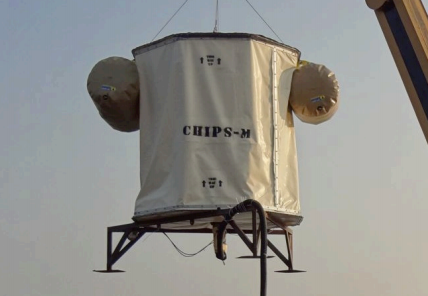
\includegraphics[width=0.6\textwidth]{diagrams/5-chips/chips_m.png}
    \caption[Picture of the \chipsm detector.]
    {Picture of the \chipsm detector just before deployment. The umbilical is visable, attached to
        the bottom endcap of the detector.}
    \label{fig:chips_m}
\end{figure}

\section{The \chipsfive detector} %%%%%%%%%%%%%%%%%%%%%%%%%%%%%%%%%%%%%%%%%%%%%%%%%%%%%%%%%%%%%%%%
\label{sec:chips_detector} %%%%%%%%%%%%%%%%%%%%%%%%%%%%%%%%%%%%%%%%%%%%%%%%%%%%%%%%%%%%%%%%%%%%%%%

- The chips-5 detector is the first of these units, at 25m in diameter and 12m tall.
- This leads to a fiducial volume of ~5kton
- Will be initially deployed into the Wentworth Pit 2W in northen minnesota, which is 7 mrad
off-axis of the numi beam.
- Also deep enough to allow for ~50m of everburden of water to reduce the cosmic background.
- Not at the ideal location (baseline) to measure the mass hierarchy in the Numi beam.
- Can help to constrain delta-cp by measuring electron neutrino appearance.
- Physics capabilities have been studied using GLoBES, should ask Tom for a nice plot and brief
description of how it all works.
- Wentworth 2W is a disused surface iron pit (taconite ore) owned by Cliffs natural resources.
- Has advantages of having the infastrucutre in place for heavy industry, such as power and roads.
- The main Polymet mining building is less than a mile from the deployment site which was used as
a laboratory environment for building detector compoenents on site.
- located at a latitude of 47.58N and longitude of 92.13W. It is 7 mrad off the centralaxis of the
NuMI beam at a baseline of 712 km
- Water is drained from the pit in the spring to ensure it does not overflow during the summer
rainy season.
- Therefore, fluctutationsof +-3m are expected over the course of a year.
- A lighttight liner a polymer membrance is used to seperate the clean detector water from the
external pit water and isolate the detector volume.
- This detector will act as a proff of concept that the R\&D has been a success and the provide
possible improvements for future iterations.
- CHIPS will not initially have a near detector, however the use of NOVA one is possible if
required, but not important for now.
- You would really need a water cherenkov near detector, so it as simiar as possible as the far
detector.
- This allows the same event reco and PID minimising systematic uncertainties in the predicted
background at the far detector.
- Is prefered as it has the same neutrino interaction traget (water) ensuring efficiencies are
similar in both detector.
- However, it should be noted that a water cherenkov detector has never been proven in high
intensity environmenets such as the Numi beam (WTF is t2k then)

INFO: detector module
- Dimensions
- Inner surface area
- PMT diameter
- photocathode coverage in different regions
- No of PMTs
- overburden
- CR muon rate
- In-spill CR occupancy
- CR event dead time
- Veto dimensions
- Veto num PMTs
- veto photocathode coverage
- veto pmt diameter

\begin{figure} % CHIPS SUNRISE DIAGRAM %
    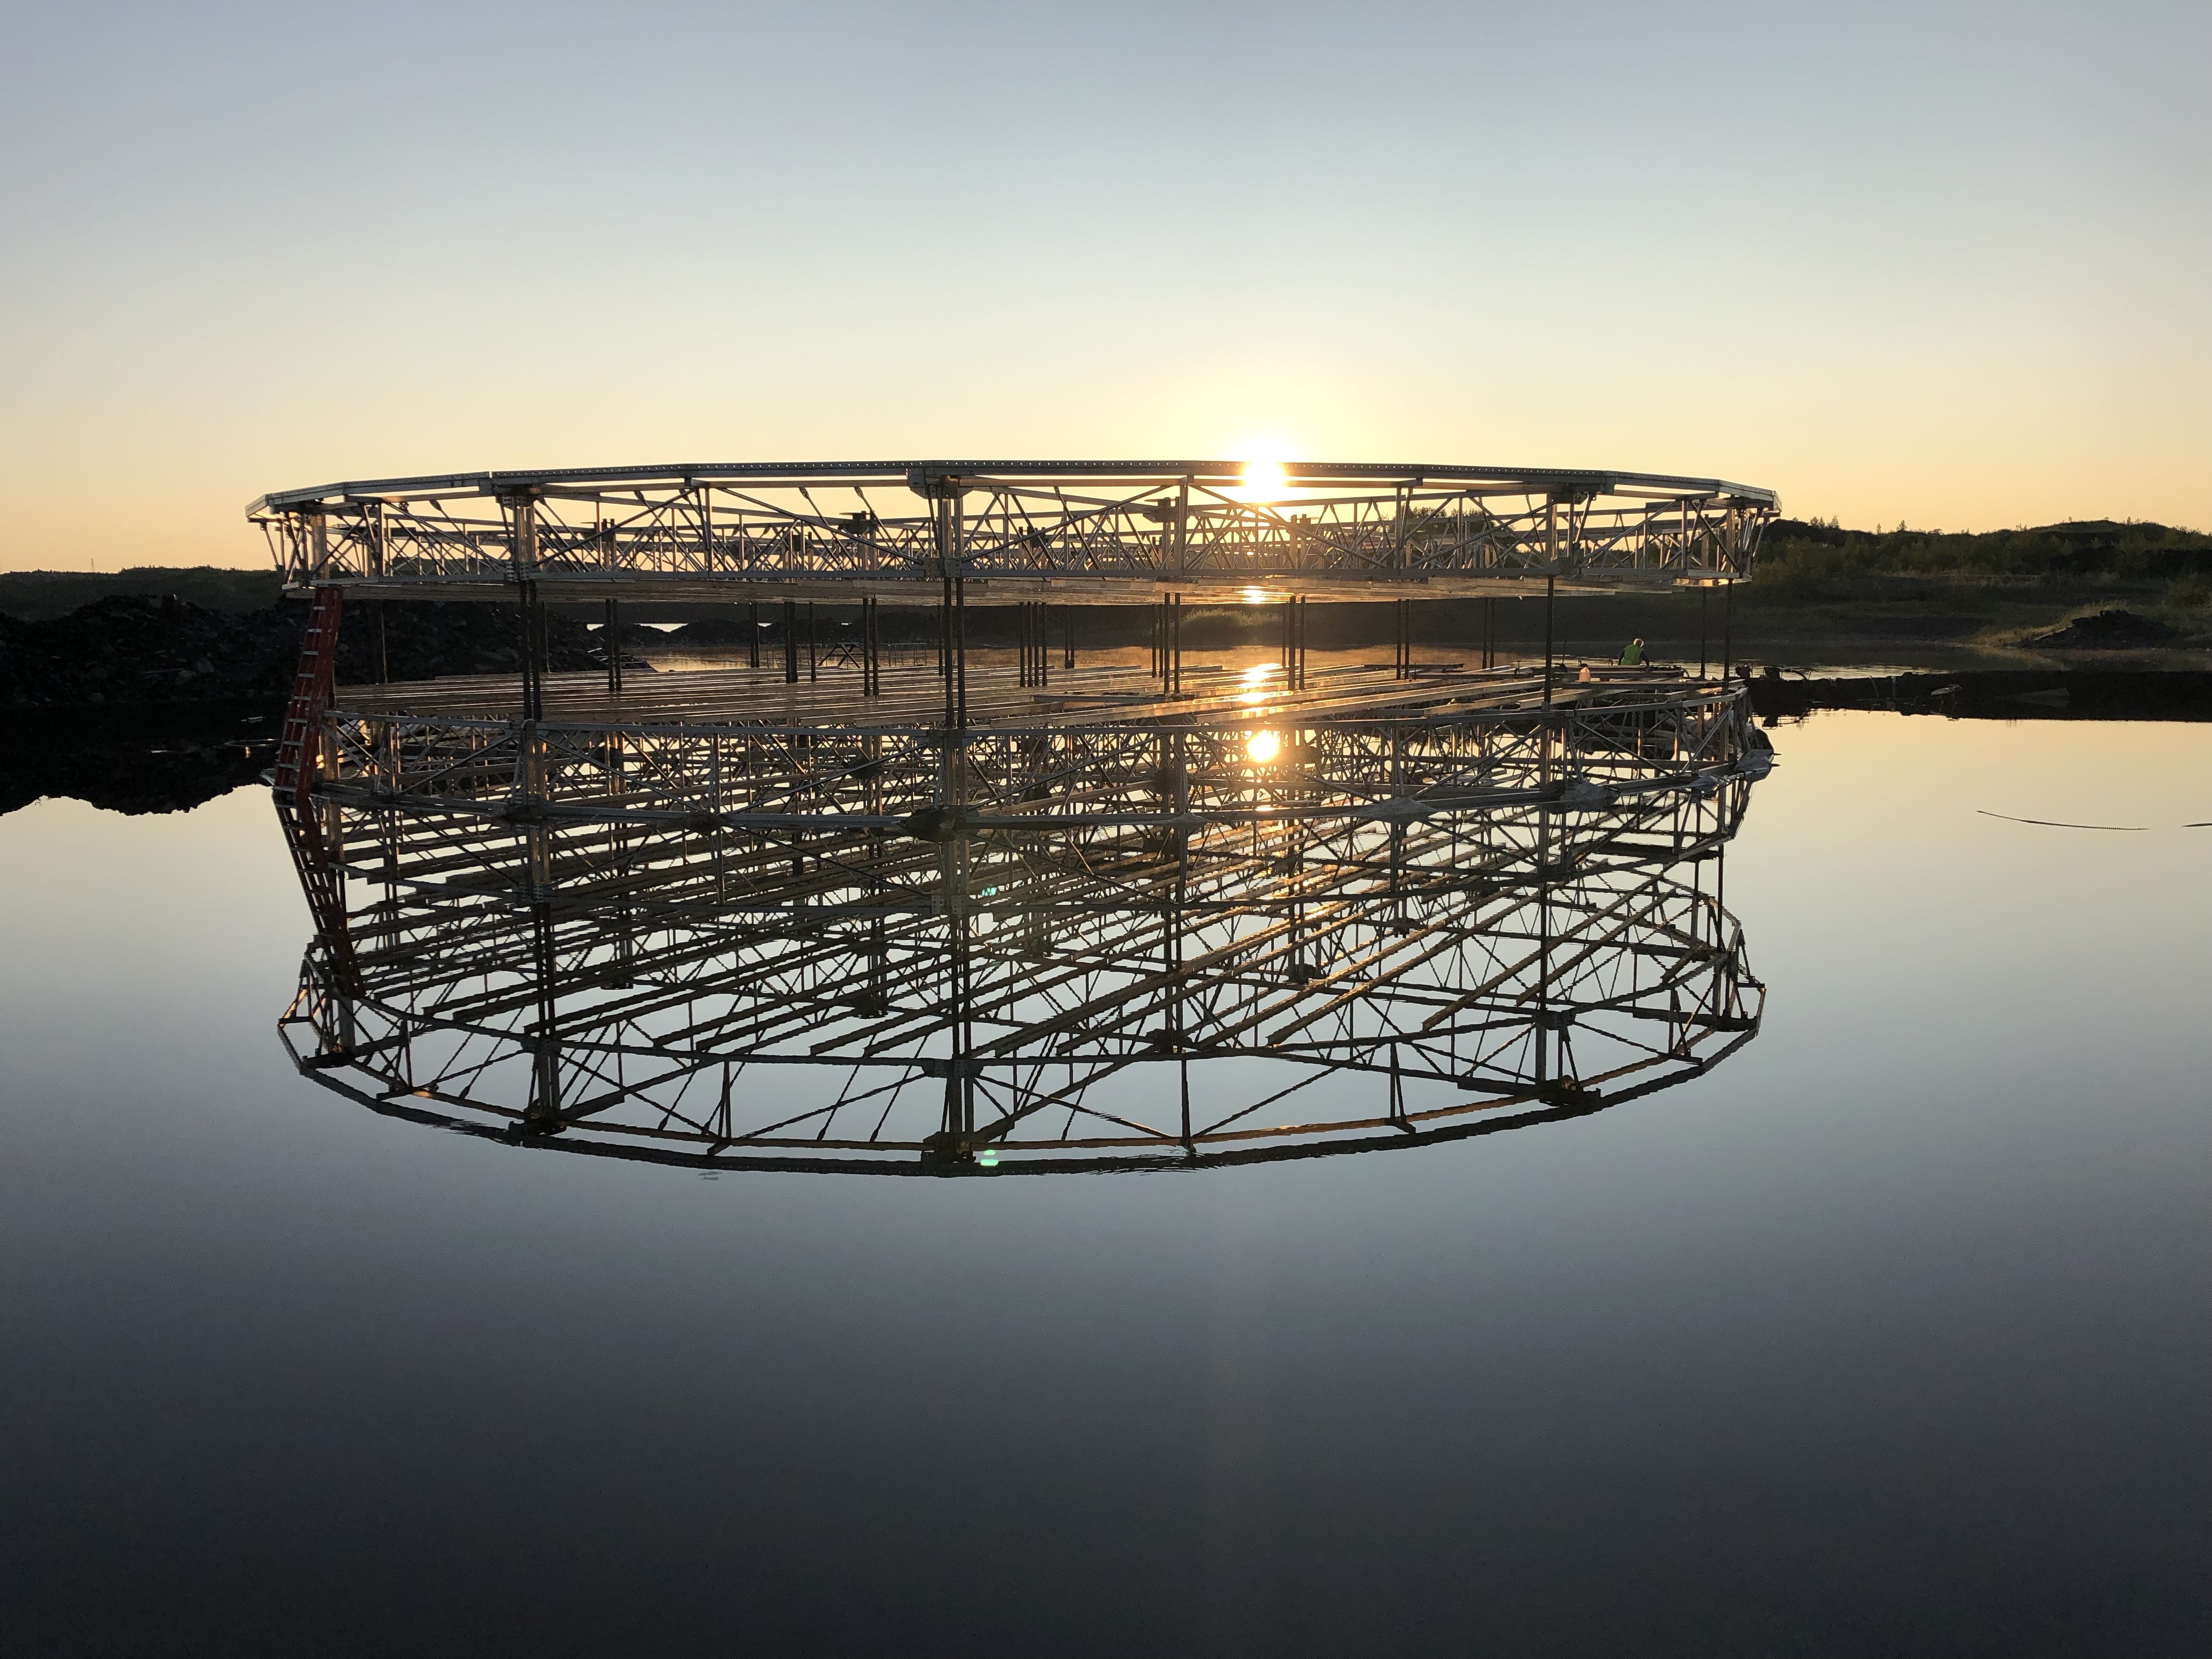
\includegraphics[width=0.6\textwidth]{diagrams/5-chips/sunrise.jpeg}
    \caption[Sunrise over the \chips detector.]
    {Sunrise over the \chips detector structure. The perfectly calm pit water
        produces the mirror effect.}
    \label{fig:sunrise}
\end{figure}

\begin{figure} % CHIPS FROM THE SKY DIAGRAM %
    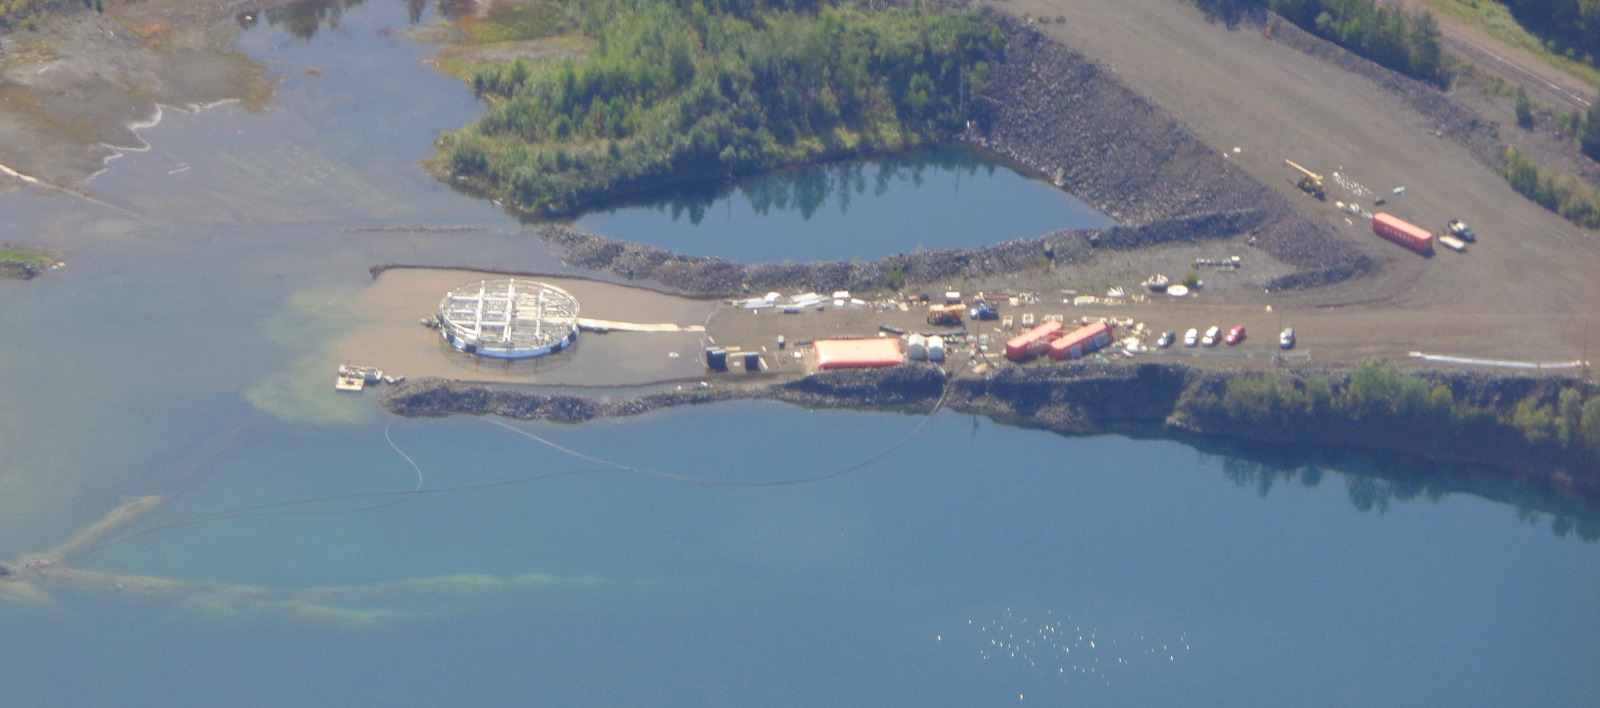
\includegraphics[width=0.6\textwidth]{diagrams/5-chips/from_the_sky.jpg}
    \caption[Picture of the \chips detector from the air.]
    {Picture of the \chips detector taken from an airplane. The Wentworth 2W pit is in the lower
        half of the image, with the half built detector, huts and construction containers
        visable.}
    \label{fig:from_the_sky}
\end{figure}

\begin{figure} % PIT DIAGRAM %
    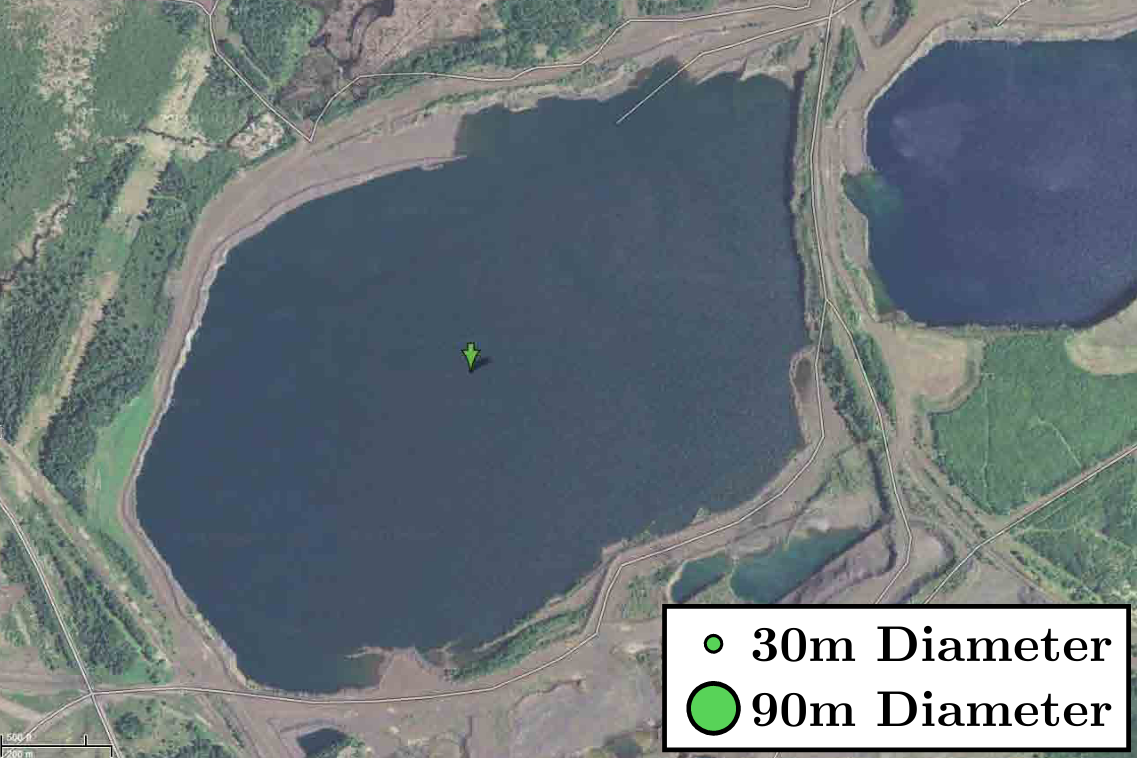
\includegraphics[width=0.6\textwidth]{diagrams/5-chips/location.png}
    \caption[Satellite view of the Wentworth 2W mine pit.]
    {Satellite view of the Wentworth 2W mine pit in northern Minnesota.
        The size markers are shown for scale. Image taken from Ref.\cite{adamson2013}.}
    \label{fig:location}
\end{figure}

\begin{figure} % PIT CONTOUR DIAGRAM %
    \includegraphics[width=0.6\textwidth]{diagrams/5-chips/contour_map.pdf}
    \caption[Topographic map of the Wentworth 2W mine pit.]
    {Topographic map of the Wentworth 2W mine pit. The contours are given in intervals of 5 feet,
        with the central areas of the pit having a depth of 50m. Image taken from
        Ref.\cite{adamson2013}.}
    \label{fig:contour_map}
\end{figure}

\begin{figure} % CHIPS LOCATION IN NUMI DIAGRAM %
    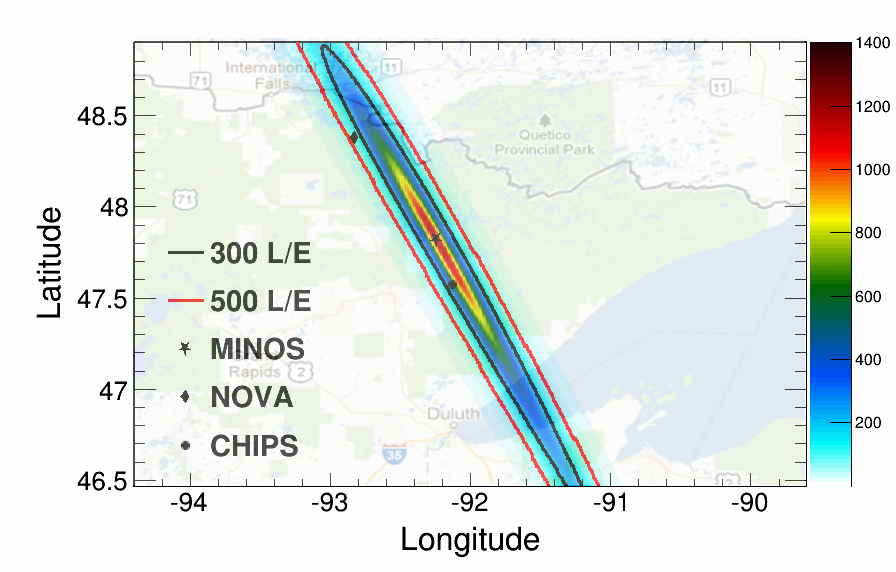
\includegraphics[width=0.6\textwidth]{diagrams/5-chips/numi_map.png}
    \caption[Map of detector locations in the \numi beam.]
    {Map of the \chips, \nova and \minos locations in the \numi beam showing the expected
        neutrino event rates, assuming no oscillations. Lines of constant L/E are shown by the
        contours. Image taken from Ref.\cite{adamson2013}.}
    \label{fig:numi_map}
\end{figure}

\subsection{Structure} %%%%%%%%%%%%%%%%%%%%%%%%%%%%%%%%%%%%%%%%%%%%%%%%%%%%%%%%%%%%%%%%%%%%%%%%%%%
\label{sec:chips_detector_structure} %%%%%%%%%%%%%%%%%%%%%%%%%%%%%%%%%%%%%%%%%%%%%%%%%%%%%%%%%%%%%

\begin{figure} % CHIPS RENDER 1 DIAGRAM %
    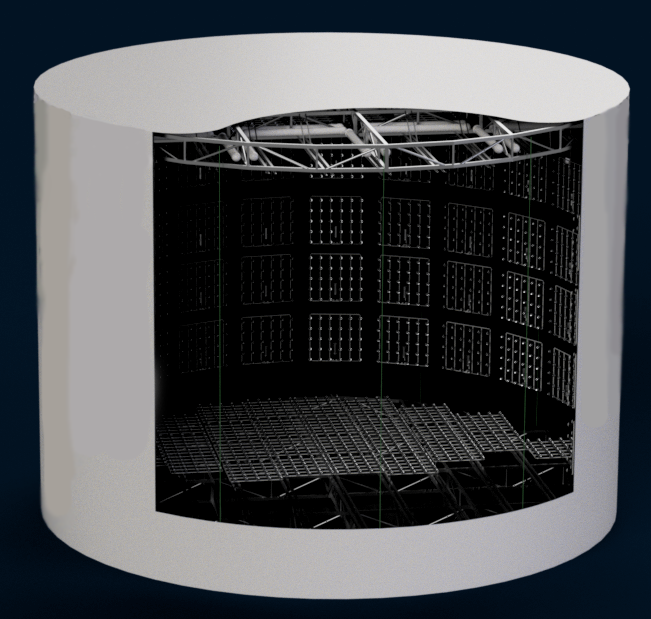
\includegraphics[width=0.6\textwidth]{diagrams/5-chips/chips_render_1.png}
    \caption[Graphical rendering of the \chipsfive detector with liner cutaway.]
    {Graphical rendering of the \chipsfive detector with a section of the liner cutaway.
        The bottom endcap and wall planes are visable,
        as well as the top endcap structure and floatation.}
    \label{fig:chips_render_1}
\end{figure}

\begin{figure} % CHIPS RENDER 2 DIAGRAM %
    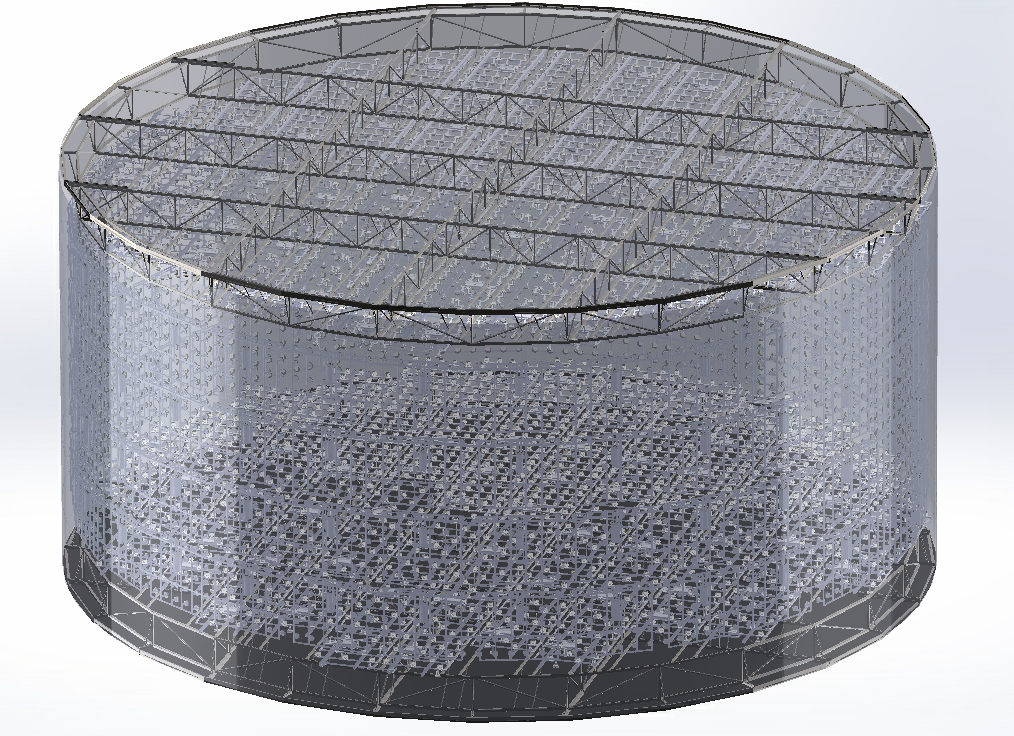
\includegraphics[width=0.6\textwidth]{diagrams/5-chips/chips_render_2.png}
    \caption[Graphical rendering of the \chipsfive detector structure.]
    {Graphical rendering of the \chipsfive detector structure.}
    \label{fig:chips_render_2}
\end{figure}

\subsection{Instrumentation} %%%%%%%%%%%%%%%%%%%%%%%%%%%%%%%%%%%%%%%%%%%%%%%%%%%%%%%%%%%%%%%%%%%%%
\label{sec:chips_detector_instrumentation} %%%%%%%%%%%%%%%%%%%%%%%%%%%%%%%%%%%%%%%%%%%%%%%%%%%%%%%

km3net 2.0 ref in \cite{adrian2016}
Icecube DOM paper \cite{hanson2006}

DIAGRAM: POM diagram
REF: Km3net optical module paper
REF: Nemo-3 PMT paper
- CHIPS uses high quantum efficiency PMTs from Hamamatsu
REF: Get hamamatsu PMT reference
- We will talk in detail about DAQ in the following chapter
- For calibration "flashers" are built into the detector to allow for known location light
generation to calibrate final PMT positions and time resolutuions.

\begin{figure} % PMT ASSEMBLY DIAGRAM %
    \centering
    \subcaptionbox{pmt disassembled\label{fig:pmt_disassembled}}{%
        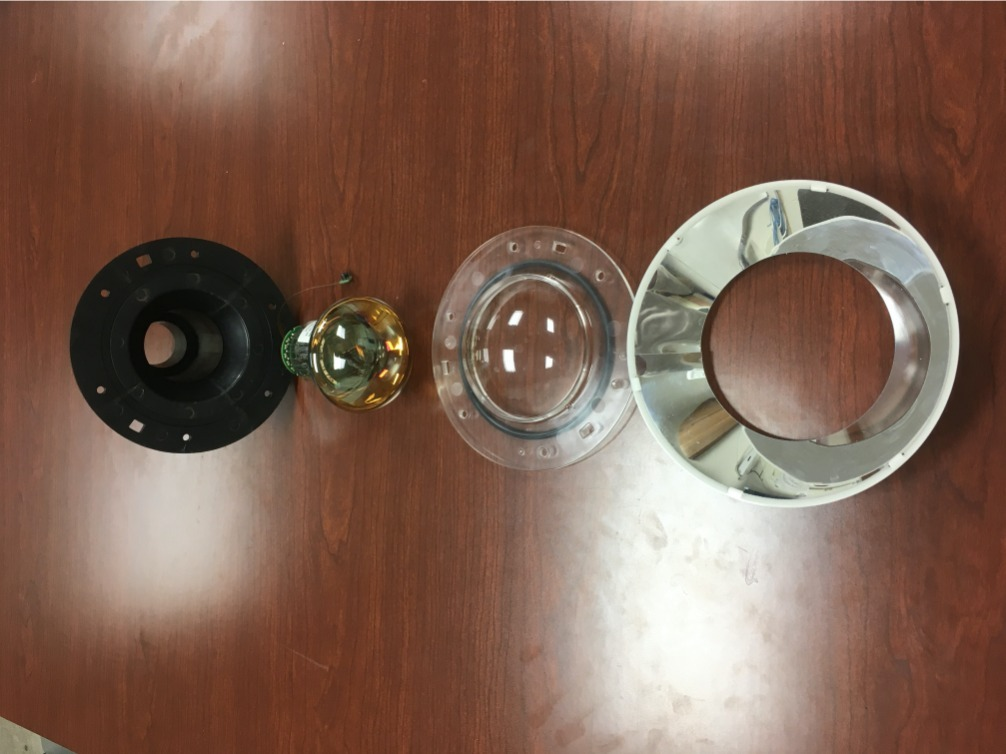
\includegraphics[height=5cm]{diagrams/5-chips/pmt_disassembled.jpg}%
    }
    \quad
    \subcaptionbox{pmt assembled\label{fig:pmt_assembled}}{%
        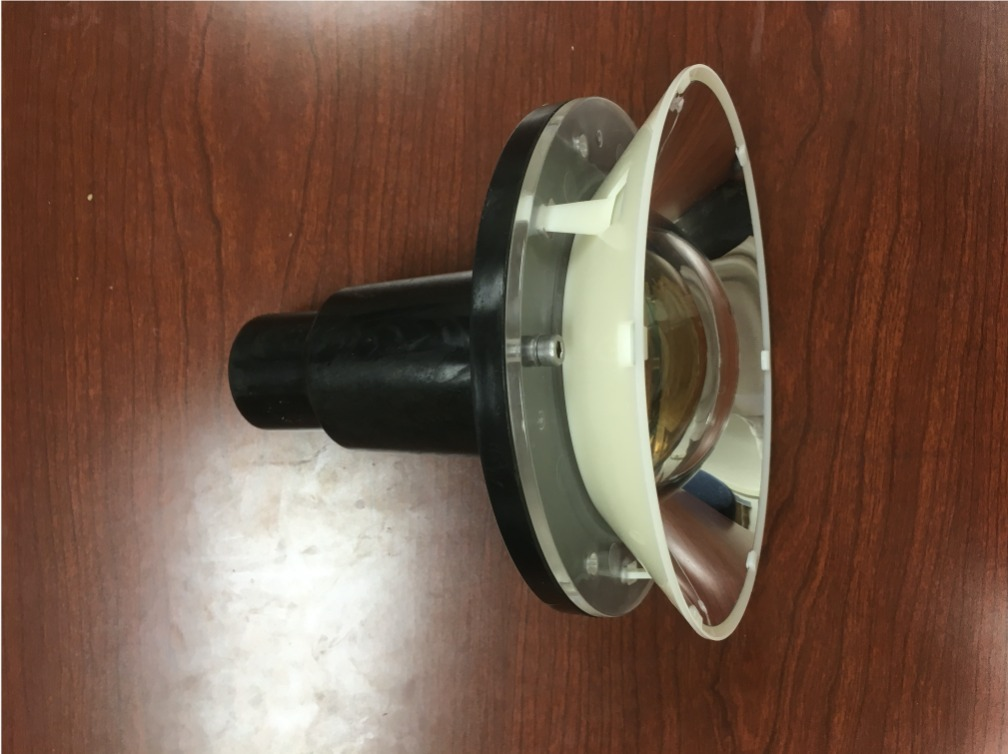
\includegraphics[height=5cm]{diagrams/5-chips/pmt_assembled.jpg}%
    }
    \caption[The caption]
    {The caption}
\end{figure}

\begin{figure} % NIKHEF PLANE DIAGRAM %
    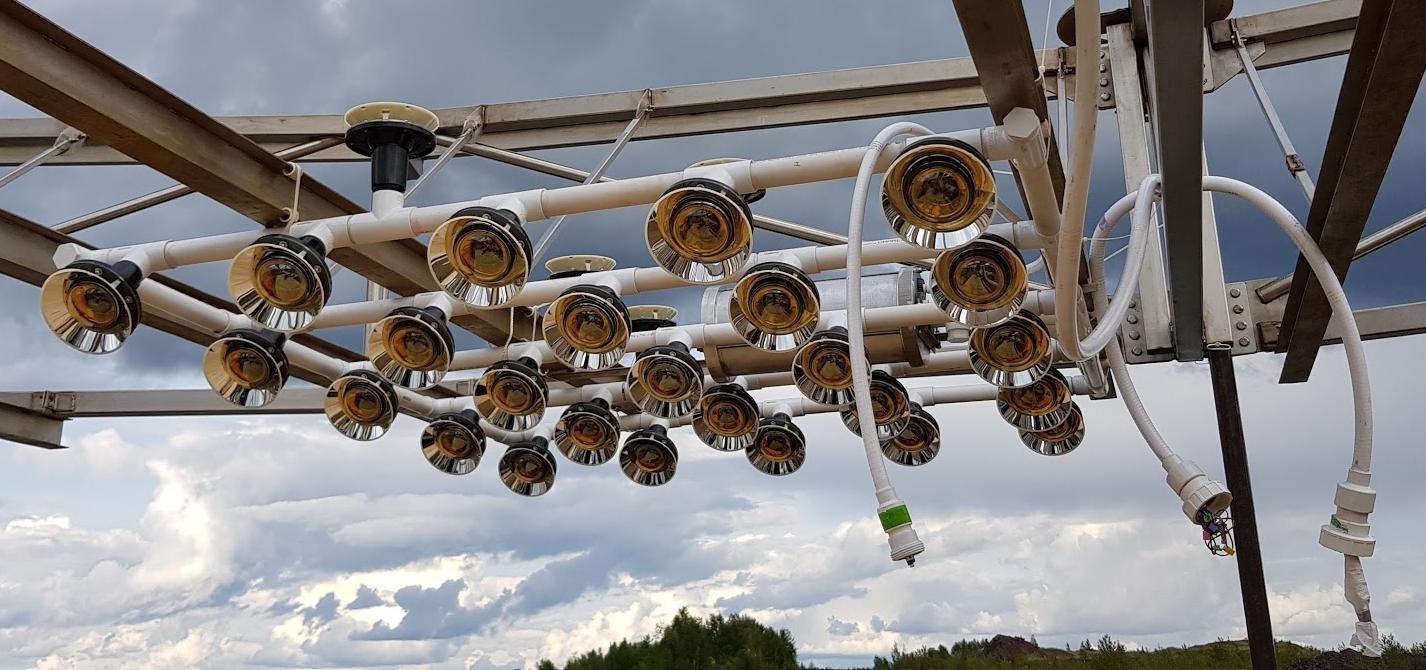
\includegraphics[width=0.8\textwidth]{diagrams/5-chips/single_plane.jpg}
    \caption[Picture of a single `Nikhef' plane.]
    {Picture of a single `Nikhef' high density top endcap plane. Both the inward facing and veto
        PMTs can be seen as well as the planes umbilical with the green tape attached.}
    \label{fig:single_plane}
\end{figure}

\subsection{Water clarity} %%%%%%%%%%%%%%%%%%%%%%%%%%%%%%%%%%%%%%%%%%%%%%%%%%%%%%%%%%%%%%%%%%%%%%%
\label{sec:chips_detector_water} %%%%%%%%%%%%%%%%%%%%%%%%%%%%%%%%%%%%%%%%%%%%%%%%%%%%%%%%%%%%%%%%%

- Though remarkably clear the Wentworth pit water is not clean enough for the detector volume
where we require ~30m attenuation length.
- CHIPS attenuation length paper~\cite{amat2017}

\subsection{Deployment} %%%%%%%%%%%%%%%%%%%%%%%%%%%%%%%%%%%%%%%%%%%%%%%%%%%%%%%%%%%%%%%%%%%%%%%%%%
\label{sec:chips_detector_deployment} %%%%%%%%%%%%%%%%%%%%%%%%%%%%%%%%%%%%%%%%%%%%%%%%%%%%%%%%%%%%

DIAGRAM: Floating dock diagram
DIAGRAM: Deployment diagram
- How it can grow if needed

\subsection{Current status} %%%%%%%%%%%%%%%%%%%%%%%%%%%%%%%%%%%%%%%%%%%%%%%%%%%%%%%%%%%%%%%%%%%%%%
\label{sec:chips_detector_status} %%%%%%%%%%%%%%%%%%%%%%%%%%%%%%%%%%%%%%%%%%%%%%%%%%%%%%%%%%%%%%%%

\section{Monte Carlo event generation and simulation} %%%%%%%%%%%%%%%%%%%%%%%%%%%%%%%%%%%%%%%%%%%%
\label{sec:chips_monte_carlo} %%%%%%%%%%%%%%%%%%%%%%%%%%%%%%%%%%%%%%%%%%%%%%%%%%%%%%%%%%%%%%%%%%%%

\subsection{Beam event generation} %%%%%%%%%%%%%%%%%%%%%%%%%%%%%%%%%%%%%%%%%%%%%%%%%%%%%%%%%%%%%%%
\label{sec:chips_monte_carlo_beam} %%%%%%%%%%%%%%%%%%%%%%%%%%%%%%%%%%%%%%%%%%%%%%%%%%%%%%%%%%%%%%%

\begin{figure} % CHIPS FLUX DIAGRAM %
    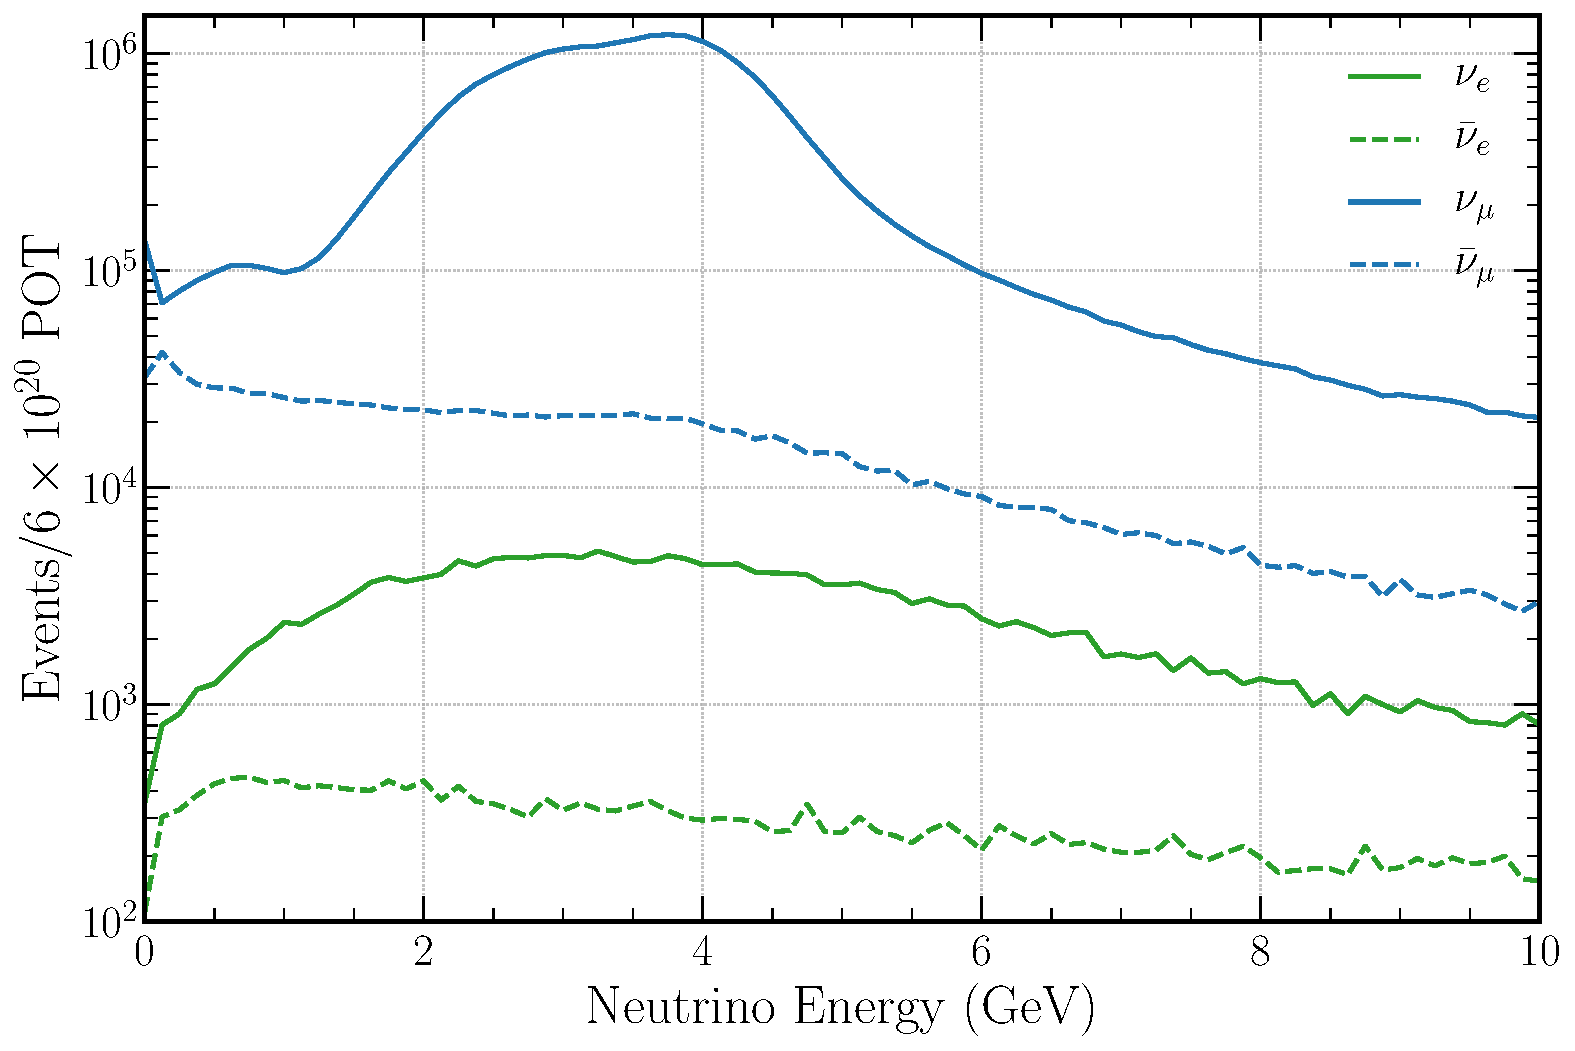
\includegraphics[width=0.6\textwidth]{diagrams/5-chips/flux.pdf}
    \caption[NuMI neutrino flux at CHIPS.]
    {The NuMI beam neutrino flux with cross-sections applied at the CHIPS detector location. Shown
        are the seperate contributions from the different neutrino types and sign. No oscillations
        have been applied.}
    \label{fig:flux}
\end{figure}

\begin{figure} % XSEC NUEL DIAGRAM %
    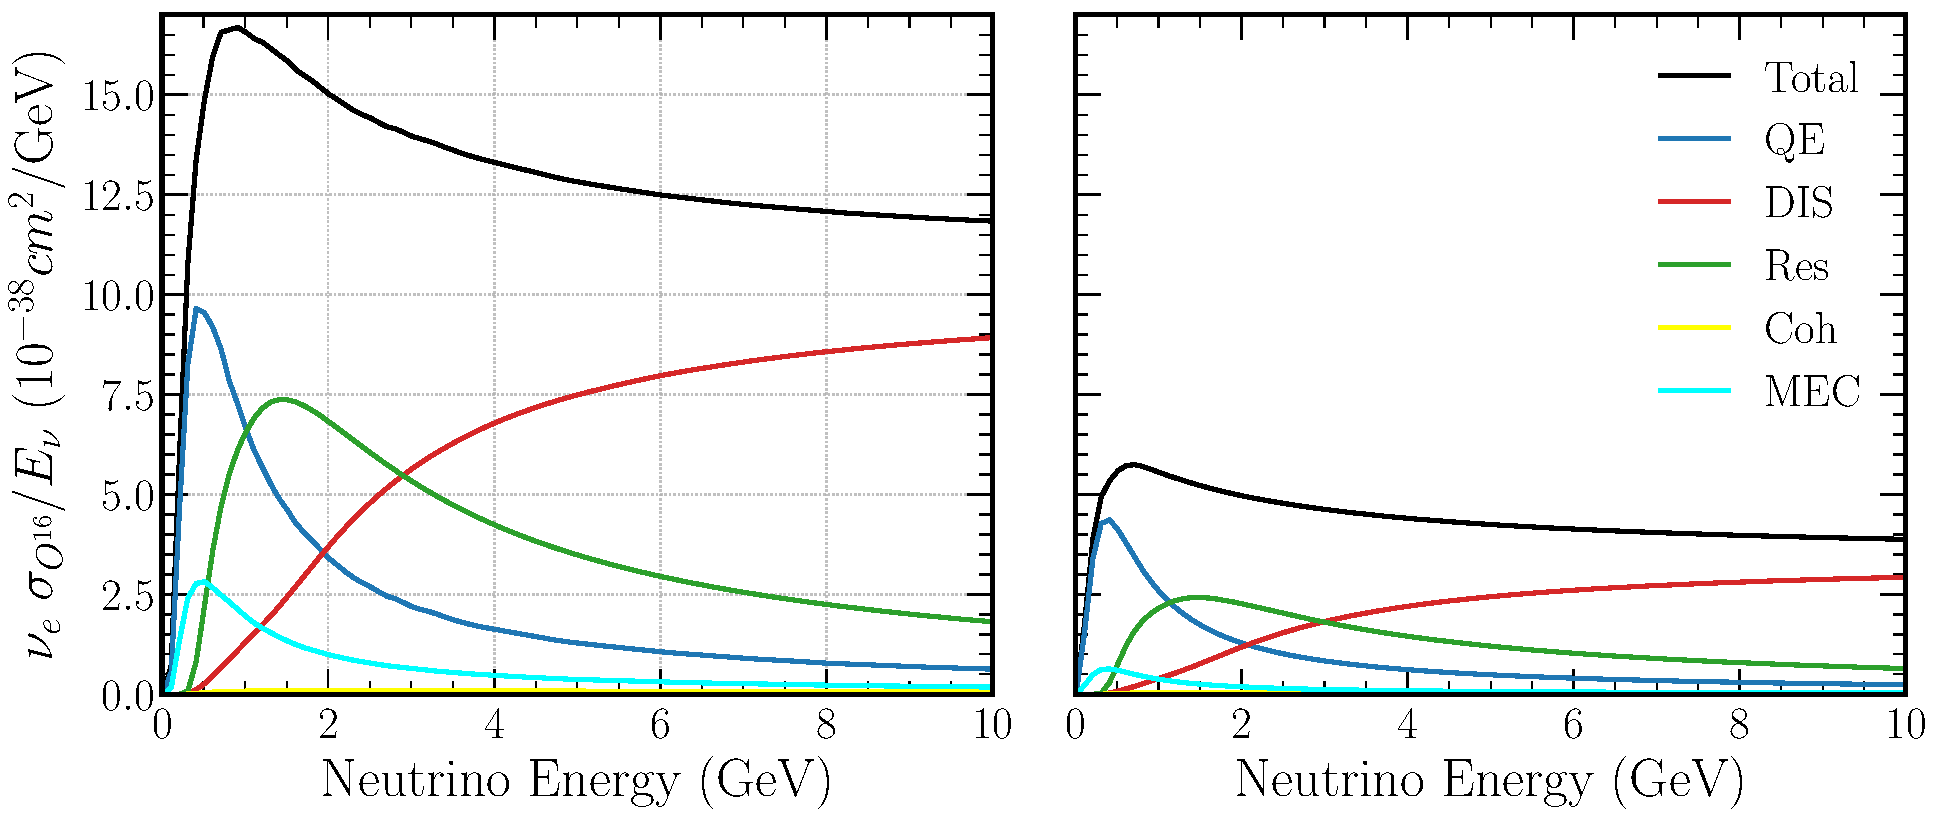
\includegraphics[width=\textwidth]{diagrams/5-chips/xsec_nu_e_O16.pdf}
    \caption[$\nu_{e}$ GENIE cross-sections.]
    {Example GENIE cross-sections used in the Monte Carlo generation of beam events. Shown are the
        $\nu_{e}$ CC (left) and NC (right) cross-sections for each of the interaction channels as
        well as the combined total.}
    \label{fig:xsec_nu_e_O16}
\end{figure}

Cosmic event rate in \cite{son2013}

- We take full advantage of the MINOS, NOVA extensive simulations of the Numi beam for use in
CHIPS.
- The tau neutrino component is negligible and not predicted by the simulation
INFO: expected number of events per year etc...

\subsection{Cosmic event generation} %%%%%%%%%%%%%%%%%%%%%%%%%%%%%%%%%%%%%%%%%%%%%%%%%%%%%%%%%%%%%
\label{sec:chips_monte_carlo_cosmic} %%%%%%%%%%%%%%%%%%%%%%%%%%%%%%%%%%%%%%%%%%%%%%%%%%%%%%%%%%%%%

DIAGRAM: expected cosmic rate at different height plot
DIAGRAM: Cosmic rate given the water overburden diagram

\begin{figure} % COSMICS AROUND DETECTOR DIAGRAM %
    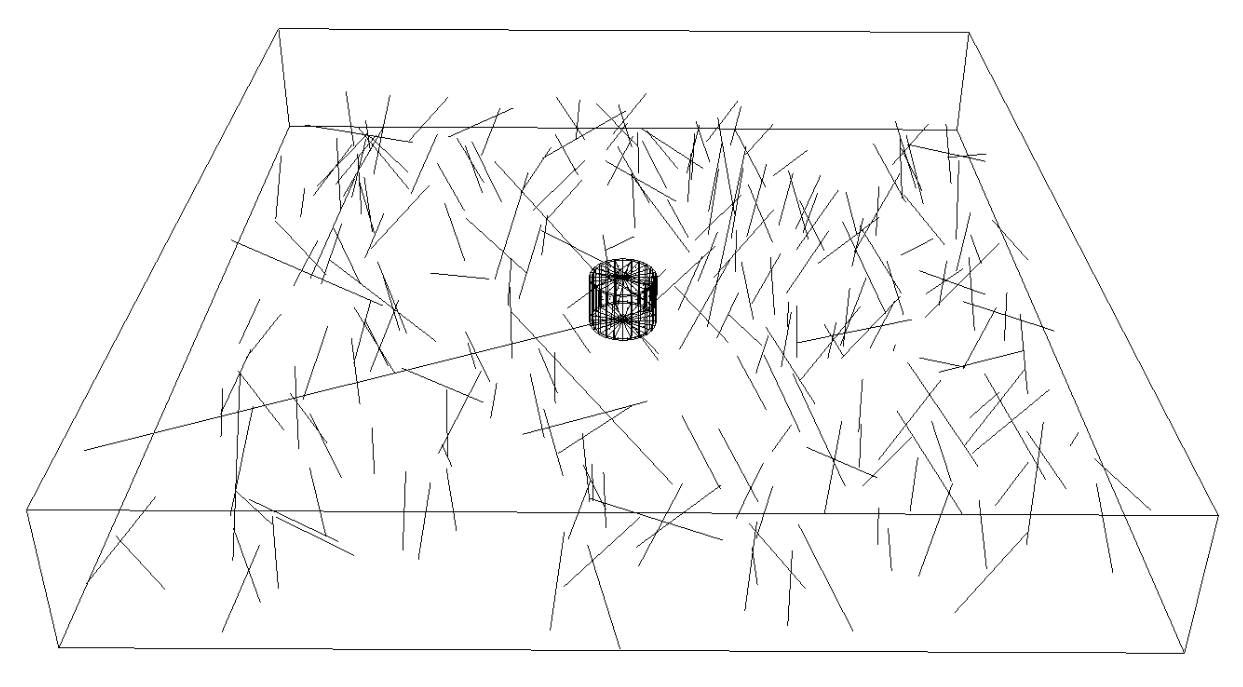
\includegraphics[width=0.8\textwidth]{diagrams/5-chips/cosmics.png}
    \caption[Cosmic muon rays around the CHIPS detector]
    {Simulated cosmic muon rays around the CHIPS detector. Note how they are generated within a
        box.}
    \label{fig:cosmics}
\end{figure}

\subsection{Detector simulation} %%%%%%%%%%%%%%%%%%%%%%%%%%%%%%%%%%%%%%%%%%%%%%%%%%%%%%%%%%%%%%%%%
\label{sec:chips_monte_carlo_sim} %%%%%%%%%%%%%%%%%%%%%%%%%%%%%%%%%%%%%%%%%%%%%%%%%%%%%%%%%%%%%%%%

\begin{figure} % SIMULATED EVENT DISPLAY DIAGRAM %
    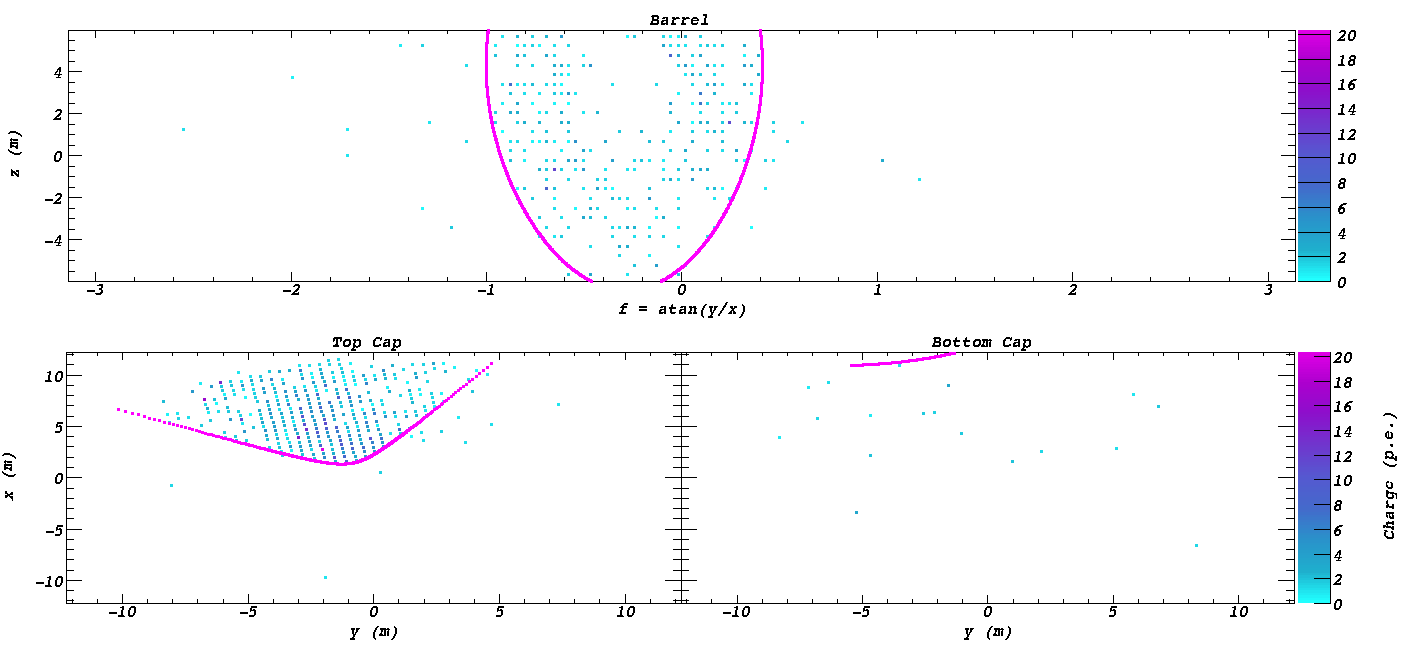
\includegraphics[width=\textwidth]{diagrams/5-chips/sim_event.png}
    \caption[sim event short]
    {$\nu_{\mu}$ CC quasi-elastic event with a single muon final state particle of energy
        1770.24 MeV}
    \label{fig:sim_event}
\end{figure}

\begin{figure} % DIGI DIAGRAM %
    \centering
    \subcaptionbox{\label{fig:digi_method}}{%
        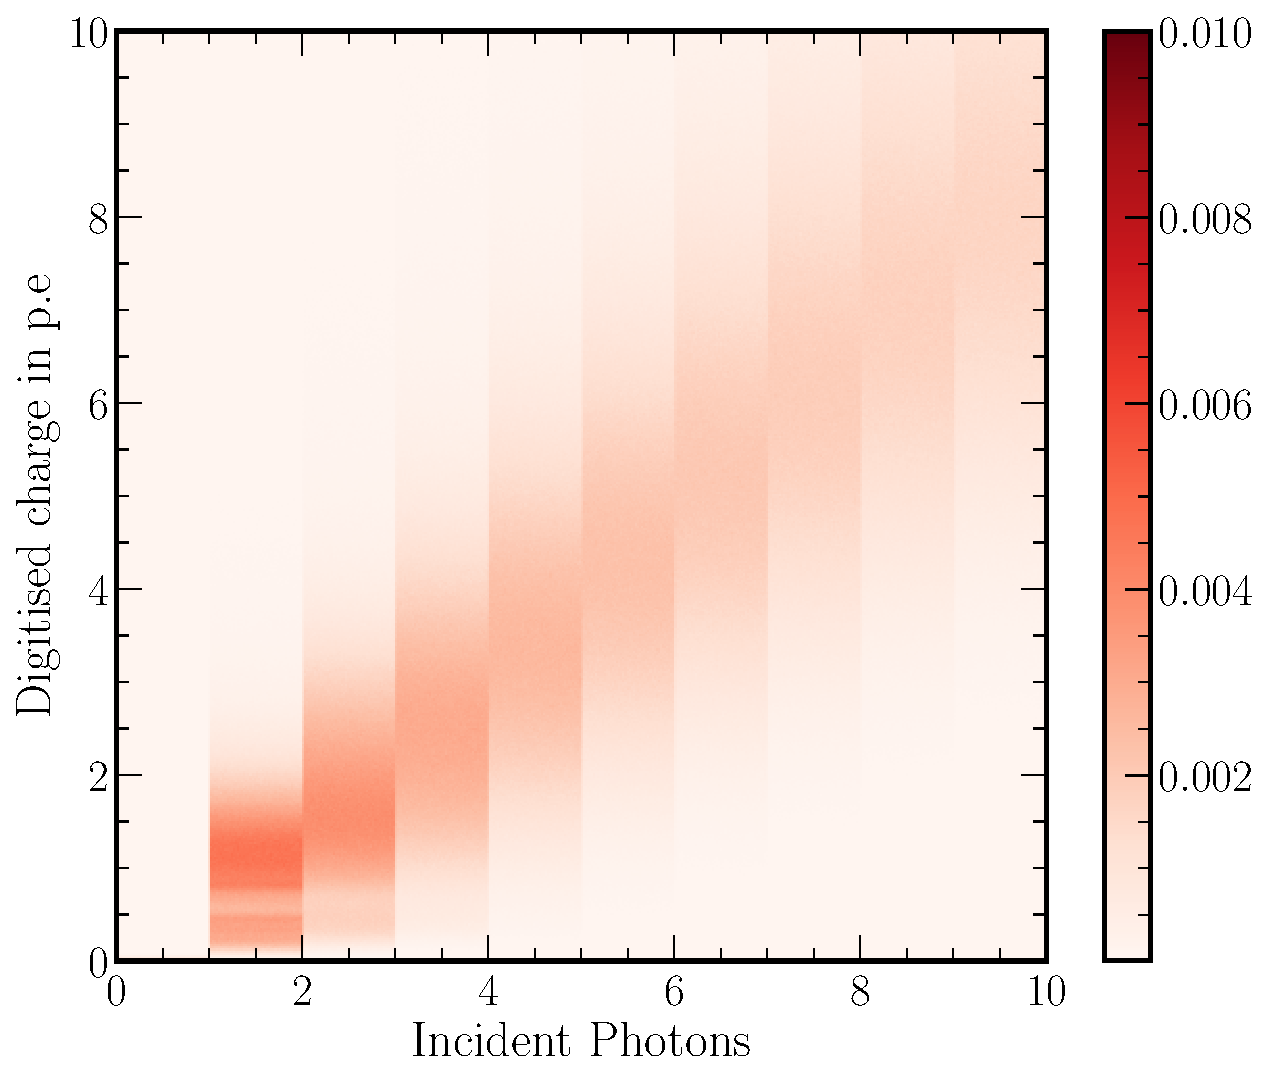
\includegraphics[height=6cm]{diagrams/5-chips/digi_method.pdf}%
    }
    \quad
    \subcaptionbox{\label{fig:digi_likelihood}}{%
        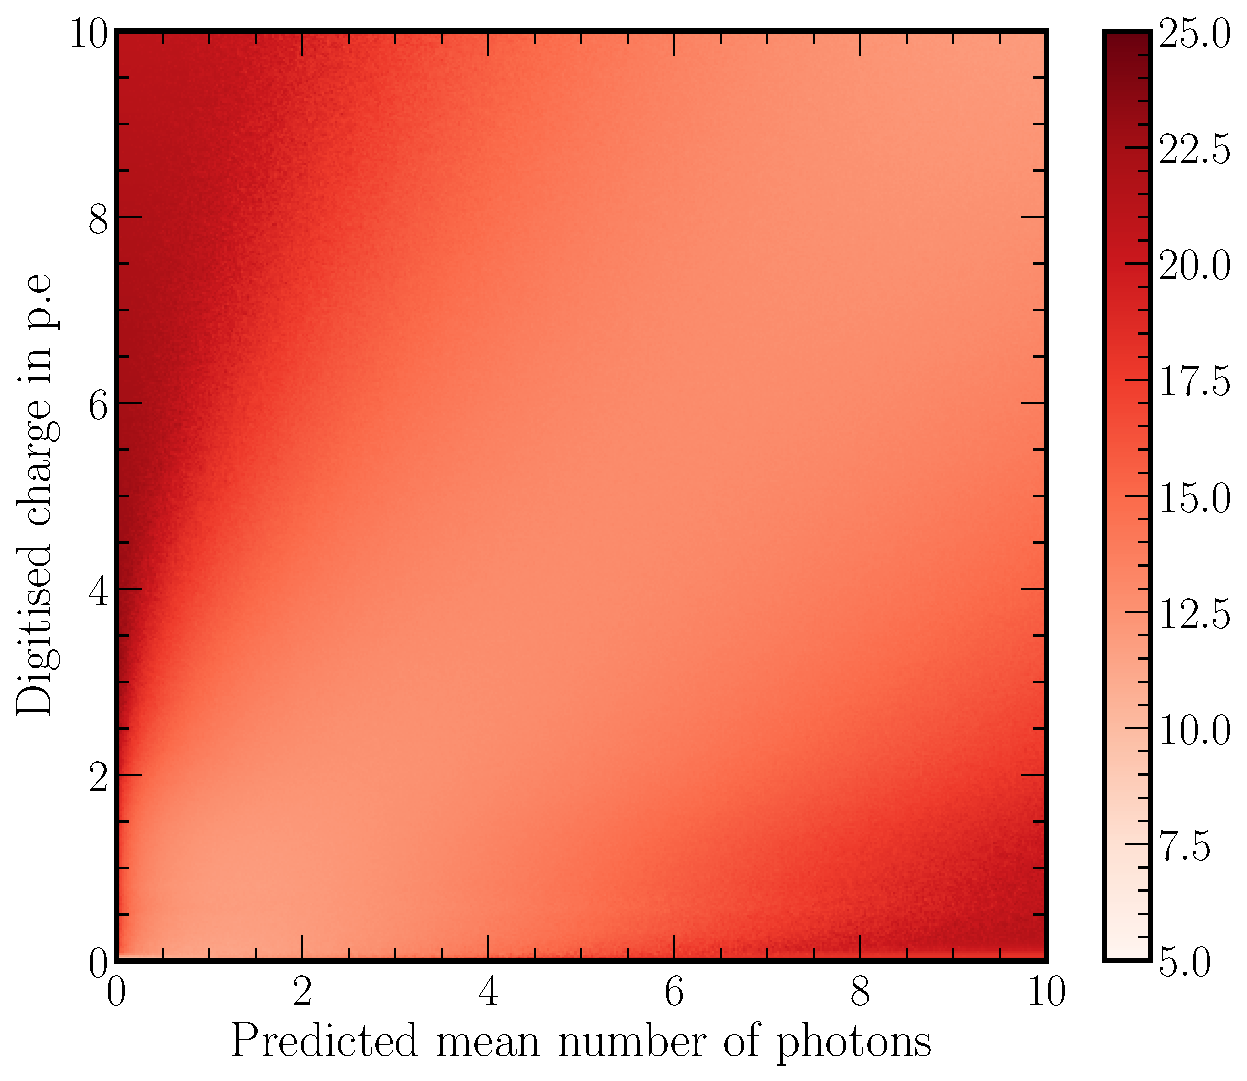
\includegraphics[height=6cm]{diagrams/5-chips/digi_likelihood.pdf}%
    }
    \caption[Simulation PMT digitisaion function.]
    {(a) Digitisation function used within the simulation to convert incident photons to measured
        digitised charge. (b) Likelihood of a measured digitised charge being caused by a number
        of photons incident on a PMT.}
\end{figure}
